\documentclass[class=article, crop=false]{standalone}\usepackage[]{graphicx}\usepackage[]{color}
%% maxwidth is the original width if it is less than linewidth
%% otherwise use linewidth (to make sure the graphics do not exceed the margin)
\makeatletter
\def\maxwidth{ %
  \ifdim\Gin@nat@width>\linewidth
    \linewidth
  \else
    \Gin@nat@width
  \fi
}
\makeatother

\definecolor{fgcolor}{rgb}{0.196, 0.196, 0.196}
\newcommand{\hlnum}[1]{\textcolor[rgb]{0.063,0.58,0.627}{#1}}%
\newcommand{\hlstr}[1]{\textcolor[rgb]{0.063,0.58,0.627}{#1}}%
\newcommand{\hlcom}[1]{\textcolor[rgb]{0.588,0.588,0.588}{#1}}%
\newcommand{\hlopt}[1]{\textcolor[rgb]{0.196,0.196,0.196}{#1}}%
\newcommand{\hlstd}[1]{\textcolor[rgb]{0.196,0.196,0.196}{#1}}%
\newcommand{\hlkwa}[1]{\textcolor[rgb]{0.231,0.416,0.784}{#1}}%
\newcommand{\hlkwb}[1]{\textcolor[rgb]{0.627,0,0.314}{#1}}%
\newcommand{\hlkwc}[1]{\textcolor[rgb]{0,0.631,0.314}{#1}}%
\newcommand{\hlkwd}[1]{\textcolor[rgb]{0.78,0.227,0.412}{#1}}%
\let\hlipl\hlkwb

\usepackage{framed}
\makeatletter
\newenvironment{kframe}{%
 \def\at@end@of@kframe{}%
 \ifinner\ifhmode%
  \def\at@end@of@kframe{\end{minipage}}%
  \begin{minipage}{\columnwidth}%
 \fi\fi%
 \def\FrameCommand##1{\hskip\@totalleftmargin \hskip-\fboxsep
 \colorbox{shadecolor}{##1}\hskip-\fboxsep
     % There is no \\@totalrightmargin, so:
     \hskip-\linewidth \hskip-\@totalleftmargin \hskip\columnwidth}%
 \MakeFramed {\advance\hsize-\width
   \@totalleftmargin\z@ \linewidth\hsize
   \@setminipage}}%
 {\par\unskip\endMakeFramed%
 \at@end@of@kframe}
\makeatother

\definecolor{shadecolor}{rgb}{.97, .97, .97}
\definecolor{messagecolor}{rgb}{0, 0, 0}
\definecolor{warningcolor}{rgb}{1, 0, 1}
\definecolor{errorcolor}{rgb}{1, 0, 0}
\newenvironment{knitrout}{}{} % an empty environment to be redefined in TeX

\usepackage{alltt}
\ifstandalone
\usepackage{../../haziq_article}
\fi





\IfFileExists{upquote.sty}{\usepackage{upquote}}{}
\begin{document}

\subsection{Fisher's iris data}

We will look at Fisher's iris data set as a toy example. There are originally three categories, but we combined the last two categories, so it is now only Setosa flowers and the rest. The four covariates give various measurements of the flowers.

\begin{knitrout}
\definecolor{shadecolor}{rgb}{1, 1, 1}\color{fgcolor}\begin{kframe}
\begin{verbatim}
## 'data.frame':	150 obs. of  5 variables:
##  $ Sepal.Length: num  5.1 4.9 4.7 4.6 5 5.4 4.6 5 4.4 4.9 ...
##  $ Sepal.Width : num  3.5 3 3.2 3.1 3.6 3.9 3.4 3.4 2.9 3.1 ...
##  $ Petal.Length: num  1.4 1.4 1.3 1.5 1.4 1.7 1.4 1.5 1.4 1.5 ...
##  $ Petal.Width : num  0.2 0.2 0.2 0.2 0.2 0.4 0.3 0.2 0.2 0.1 ...
##  $ Species     : Factor w/ 3 levels "setosa","versicolor",..: 1 1 1 ..
\end{verbatim}
\end{kframe}
\end{knitrout}
\begin{knitrout}
\definecolor{shadecolor}{rgb}{1, 1, 1}\color{fgcolor}

{\centering 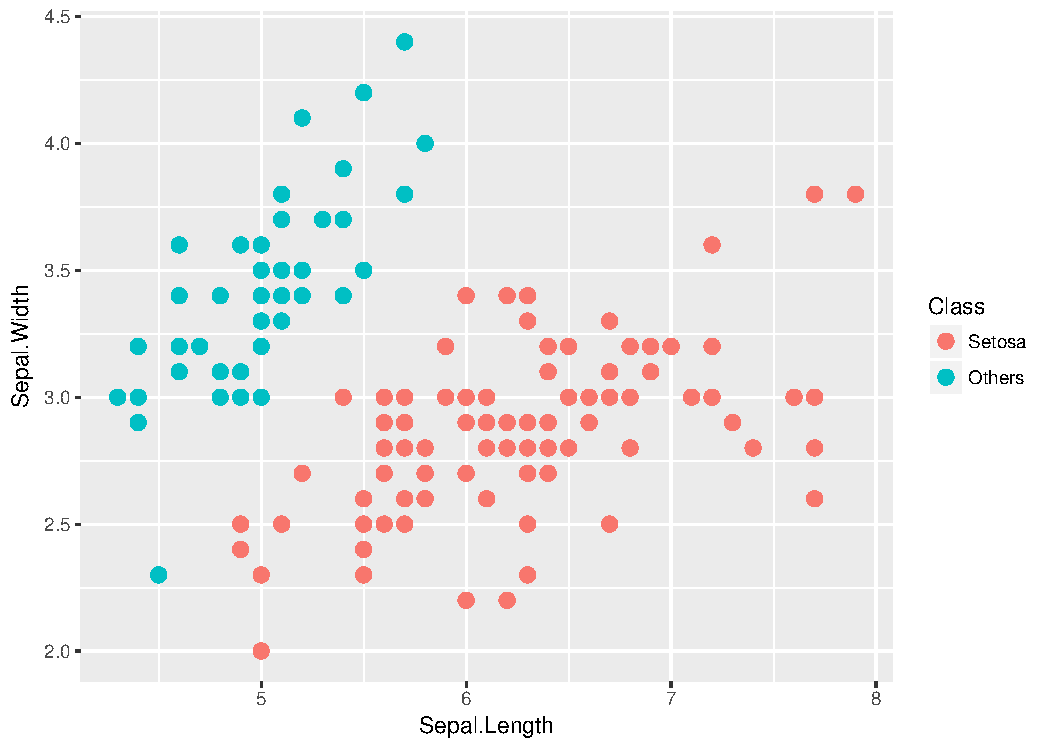
\includegraphics[width=\maxwidth]{figure/iris_plot1-1} 

}



\end{knitrout}

Fitting the probit I-prior model doesn't long at all (almost instantly). The VB-EM algorithm was run for 100 iterations. However, it is seen that it converges after just 30 iterations.

\begin{knitrout}
\definecolor{shadecolor}{rgb}{1, 1, 1}\color{fgcolor}\begin{kframe}
\begin{alltt}
\hlkwd{system.time}\hlstd{(mod} \hlkwb{<-} \hlkwd{iprobit}\hlstd{(y, X,} \hlkwc{silent} \hlstd{=} \hlnum{TRUE}\hlstd{,} \hlkwc{maxit} \hlstd{=} \hlnum{100}\hlstd{))}
\end{alltt}
\begin{verbatim}
##    user  system elapsed 
##   0.987   0.028   1.018
\end{verbatim}
\begin{alltt}
\hlkwd{print}\hlstd{(mod)}
\end{alltt}
\begin{verbatim}
## Training error rate: 0.00 %
\end{verbatim}
\end{kframe}
\end{knitrout}

\begin{knitrout}
\definecolor{shadecolor}{rgb}{1, 1, 1}\color{fgcolor}

{\centering 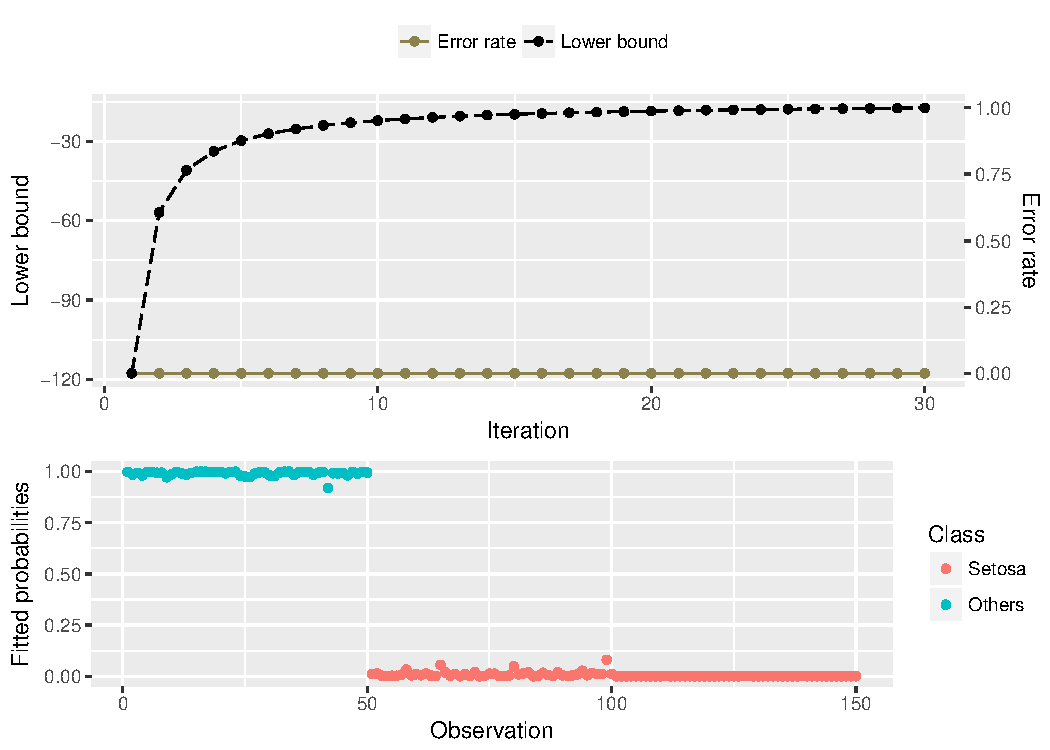
\includegraphics[width=\maxwidth]{figure/iris_plot2-1} 

}



\end{knitrout}

\subsection{Ionosphere data}

Data was obtained from \url{https://archive.ics.uci.edu/ml/datasets/Ionosphere}. This radar data was collected by a system in Goose Bay, Labrador. This system consists of a phased array of 16 high-frequency antennas with a total transmitted power on the order of 6.4 kW. The targets were free electrons in the ionosphere. ``Good'' radar returns are those showing evidence of some type of structure in the ionosphere. ``Bad'' returns are those that do not; their signals pass through the ionosphere. Received signals were processed using an autocorrelation function whose arguments are the time of a pulse and the pulse number. There were 17 pulse numbers for the Goose Bay system. Instances in this databse are described by 2 attributes per pulse number, corresponding to the complex values returned by the function resulting from the complex electromagnetic signal.

In total, there are 350 observations, and 34 covariates. Of the 350 observations, 126 were bad signals and the rest were good. Convergence was achieved pretty quickly $-$ only after about 12 iterations.

\begin{knitrout}
\definecolor{shadecolor}{rgb}{1, 1, 1}\color{fgcolor}\begin{kframe}
\begin{verbatim}
##   b   g 
## 126 224
\end{verbatim}
\end{kframe}
\end{knitrout}

We randomly split the data into a training set of size 200, and the remaining is used for validation. We obtain a training error rate of zero, but also a test error rate of 7.33\%. The FBM kernel was used.

\begin{knitrout}
\definecolor{shadecolor}{rgb}{1, 1, 1}\color{fgcolor}\begin{kframe}
\begin{alltt}
\hlstd{mod} \hlkwb{<-} \hlkwd{iprobit}\hlstd{(y.train, X.train,} \hlkwc{kernel} \hlstd{=} \hlstr{"FBM"}\hlstd{,} \hlkwc{silent} \hlstd{=} \hlnum{TRUE}\hlstd{)}
\hlkwd{print}\hlstd{(mod)}
\end{alltt}
\begin{verbatim}
## Training error rate: 0.00 %
\end{verbatim}
\begin{alltt}
\hlkwd{print}\hlstd{(mod, X.test, y.test)}  \hlcom{# Test error rate}
\end{alltt}
\begin{verbatim}
## Test error rate: 7.33 %
\end{verbatim}
\end{kframe}
\end{knitrout}
\begin{knitrout}
\definecolor{shadecolor}{rgb}{1, 1, 1}\color{fgcolor}\begin{kframe}
\begin{alltt}
\hlkwd{plot}\hlstd{(mod,} \hlnum{15}\hlstd{,} \hlkwc{levels} \hlstd{=} \hlkwd{c}\hlstd{(}\hlstr{"good"}\hlstd{,} \hlstr{"bad"}\hlstd{))}
\end{alltt}
\end{kframe}

{\centering 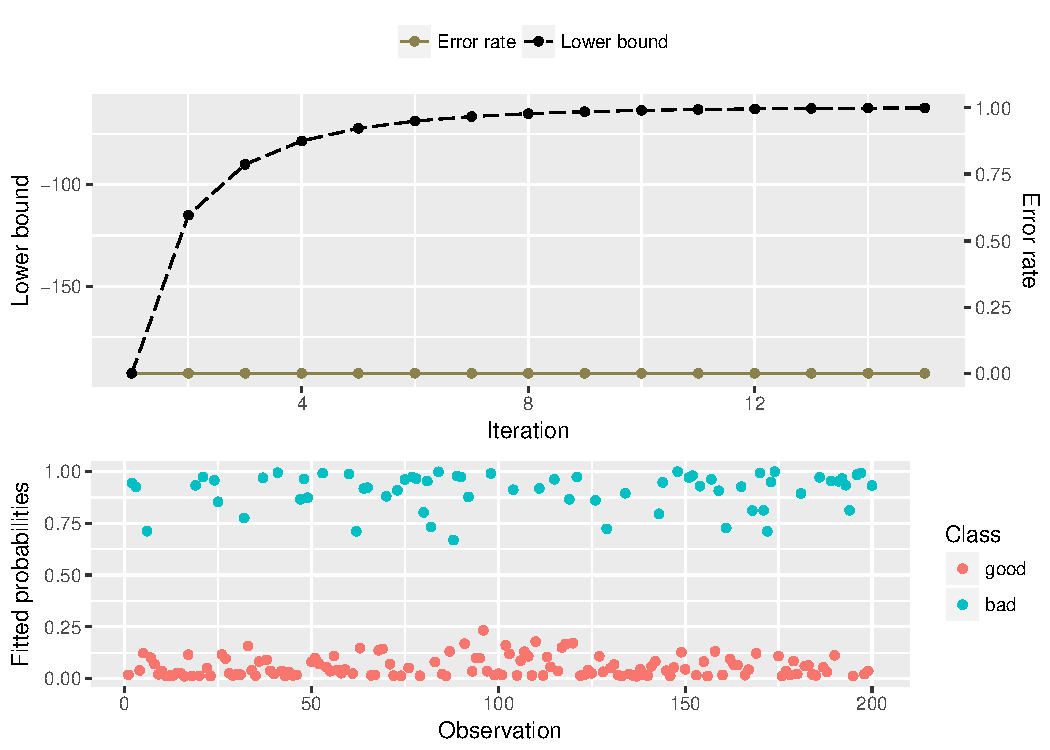
\includegraphics[width=\maxwidth]{figure/ionosphere_plot-1} 

}



\end{knitrout}

\subsection{Cardiac data}

Data was obtained from \url{https://archive.ics.uci.edu/ml/datasets/Arrhythmia}. This database contains 279 attributes, 206 of which are linear valued and the rest are nominal. Concerning the study of H. Altay Guvenir: "The aim is to distinguish between the presence and absence of cardiac arrhythmia and to classify it in one of the 16 groups. Class 1 refers to normal ECG, whereas classes 2 to 15 refers to different classes of arrhythmia, and class 16 refers to the rest of unclassified ones. For the time being, there exists a computer program that makes such a classification. However there are differences between the cardiolog's and the programs classification. Taking the cardiolog's as a gold standard we aim to minimise this difference by means of machine learning  tools."

We combined the 15 of the arrhythmia classes into a single class, and normal being a class on its own. Out of the 451 ECG observations, 245 were classed as normal, and 206 as having some form of arrhythmia. To test predictions, we split the data set into a training set of size 300, and the remaining was left for validation. We fit a probit I-prior model with an FBM kernel.

\begin{knitrout}
\definecolor{shadecolor}{rgb}{1, 1, 1}\color{fgcolor}\begin{kframe}
\begin{verbatim}
##     Normal Arrhythmia 
##        245        206
\end{verbatim}
\end{kframe}
\end{knitrout}

\begin{knitrout}
\definecolor{shadecolor}{rgb}{1, 1, 1}\color{fgcolor}\begin{kframe}
\begin{alltt}
\hlstd{mod} \hlkwb{<-} \hlkwd{iprobit}\hlstd{(y.train, X.train,} \hlkwc{kernel} \hlstd{=} \hlstr{"FBM"}\hlstd{,} \hlkwc{silent} \hlstd{= F,} \hlkwc{maxit} \hlstd{=} \hlnum{100}\hlstd{)}
\end{alltt}
\begin{verbatim}
## 
  |                                                                       
  |                                                                 |   0%
  |                                                                       
  |=                                                                |   1%
  |                                                                       
  |=                                                                |   2%
  |                                                                       
  |==                                                               |   3%
  |                                                                       
  |===                                                              |   4%
  |                                                                       
  |===                                                              |   5%
  |                                                                       
  |====                                                             |   6%
  |                                                                       
  |=====                                                            |   7%
  |                                                                       
  |=====                                                            |   8%
  |                                                                       
  |======                                                           |   9%
  |                                                                       
  |=======                                                          |  10%
  |                                                                       
  |=======                                                          |  11%
  |                                                                       
  |========                                                         |  12%
  |                                                                       
  |=========                                                        |  13%
  |                                                                       
  |=========                                                        |  14%
  |                                                                       
  |==========                                                       |  15%
  |                                                                       
  |===========                                                      |  16%
  |                                                                       
  |===========                                                      |  17%
  |                                                                       
  |============                                                     |  18%
  |                                                                       
  |============                                                     |  19%
  |                                                                       
  |=============                                                    |  20%
  |                                                                       
  |==============                                                   |  21%
  |                                                                       
  |==============                                                   |  22%
  |                                                                       
  |===============                                                  |  23%
  |                                                                       
  |================                                                 |  24%
  |                                                                       
  |================                                                 |  25%
  |                                                                       
  |=================                                                |  26%
  |                                                                       
  |==================                                               |  27%
  |                                                                       
  |==================                                               |  28%
  |                                                                       
  |===================                                              |  29%
  |                                                                       
  |====================                                             |  30%
  |                                                                       
  |====================                                             |  31%
  |                                                                       
  |=====================                                            |  32%
  |                                                                       
  |======================                                           |  33%
  |                                                                       
  |======================                                           |  34%
  |                                                                       
  |=======================                                          |  35%
  |                                                                       
  |========================                                         |  36%
  |                                                                       
  |========================                                         |  37%
  |                                                                       
  |=========================                                        |  38%
  |                                                                       
  |==========================                                       |  39%
  |                                                                       
  |==========================                                       |  40%
  |                                                                       
  |===========================                                      |  41%
  |                                                                       
  |============================                                     |  42%
  |                                                                       
  |============================                                     |  43%
  |                                                                       
  |=============================                                    |  44%
  |                                                                       
  |==============================                                   |  45%
  |                                                                       
  |==============================                                   |  46%
  |                                                                       
  |===============================                                  |  47%
  |                                                                       
  |================================                                 |  48%
  |                                                                       
  |================================                                 |  49%
  |                                                                       
  |=================================                                |  51%
  |                                                                       
  |=================================                                |  52%
  |                                                                       
  |==================================                               |  53%
  |                                                                       
  |===================================                              |  54%
  |                                                                       
  |===================================                              |  55%
  |                                                                       
  |====================================                             |  56%
## Converged after 56  iterations
\end{verbatim}
\begin{alltt}
\hlkwd{print}\hlstd{(mod)}
\end{alltt}
\begin{verbatim}
## Training error rate: 0.00 %
\end{verbatim}
\begin{alltt}
\hlkwd{print}\hlstd{(mod, X.test, y.test)}  \hlcom{# Test error rate}
\end{alltt}
\begin{verbatim}
## Test error rate: 28.67 %
\end{verbatim}
\end{kframe}
\end{knitrout}

\begin{knitrout}
\definecolor{shadecolor}{rgb}{1, 1, 1}\color{fgcolor}\begin{kframe}
\begin{alltt}
\hlkwd{plot}\hlstd{(mod,} \hlnum{15}\hlstd{,} \hlkwc{levels} \hlstd{=} \hlkwd{c}\hlstd{(}\hlstr{"Normal"}\hlstd{,} \hlstr{"Arrhythmia"}\hlstd{))}
\end{alltt}
\end{kframe}

{\centering 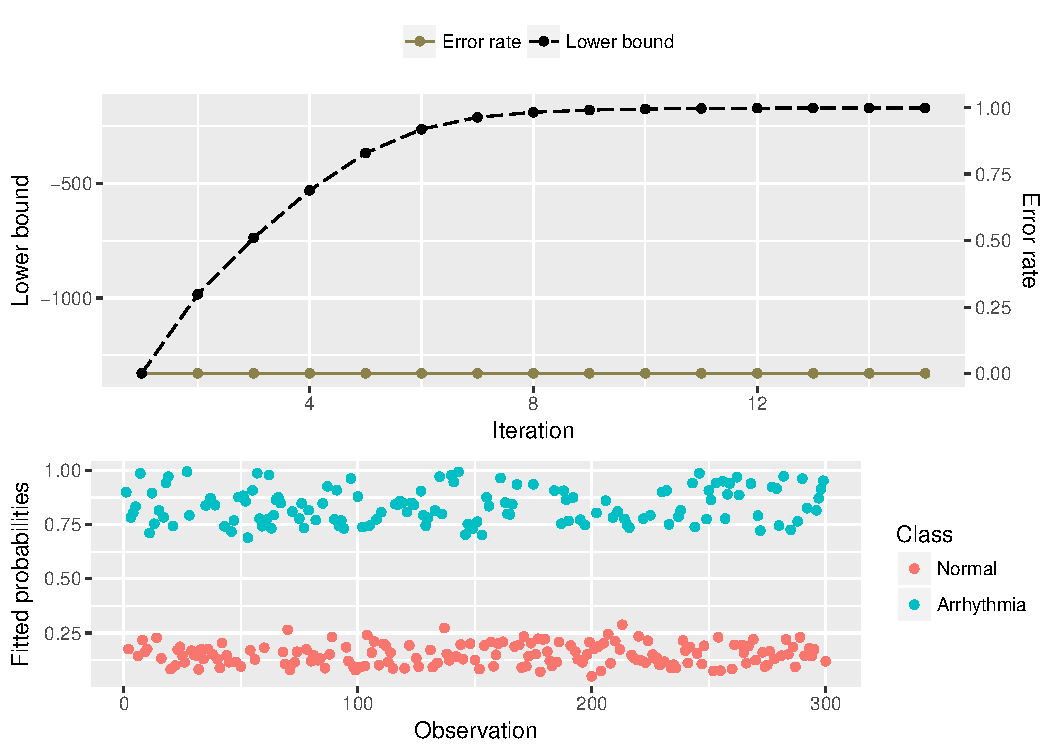
\includegraphics[width=\maxwidth]{figure/cardiac_plot-1} 

}



\end{knitrout}

\end{document}
